%\vspace{-3em}
\section{Performance}\label{sec:performance}
\vspace{-1em}
%\matthias{This is the working ProB code that we'll show as an example}
%In this section, the graph mining problem is slightly modified: we now restrict the search for a pattern to graphs that are a subgraph of a given \emph{template} graph.
%The declarative approach allows us to implement such a modification with only minimal effort.
%\VerbatimInput{original_prob_files/PositiveAndNegative.mch}
To compare the performance of higher order and first order systems, we compared the IDP system with the ProB system (which uses higher order specifications).
To this end, we used the positive examples of the Yoshida~\citep{yoshida_dataset} dataset, which is derived from biochemics, for graph mining.
First, we randomly picked an example to use as the template graph.
Next, we mined a pattern from this template, using the threshold value $N_{+} = 13$ (5\% of the size of the example set).
During the mining process, we tracked the time it takes to mine the $i=1..n$-th pattern. The results are averaged over ten runs.


The ProB model from Subsection \ref{subsection:prob} comes closest to the higher order formulation (as demonstrated in \textbf{Table} \ref{tbl:conclusion}), however, the solver support is not yet sufficient to efficiently execute the higher order graph mining model on larger datasets, i.e., currently we have not found an efficient way to mine patterns using a higher order B model. 
Consequently, from a KR point of view, we consider the higher order formulation of the graph mining problem as a challenge and goal for future solver techniques.
The key issue preventing an efficient higher order formulation lies in reifying the higher order existential quantifier inside the set comprehension. A possible future solution would be to provide a Prolog implementation for the homomorphism predicate (e.g., as a ProB external function).
For IDP, the results can be found in \textbf{Table} \ref{table:idp:averaged_results}.
%The results shown in \textbf{Fig.}~\ref{fig:ProBIDPComp} are the times needed to mine the $i$'th pattern, averaged over 10 repeats of the described process.
% \begin{figure}[thb]
% 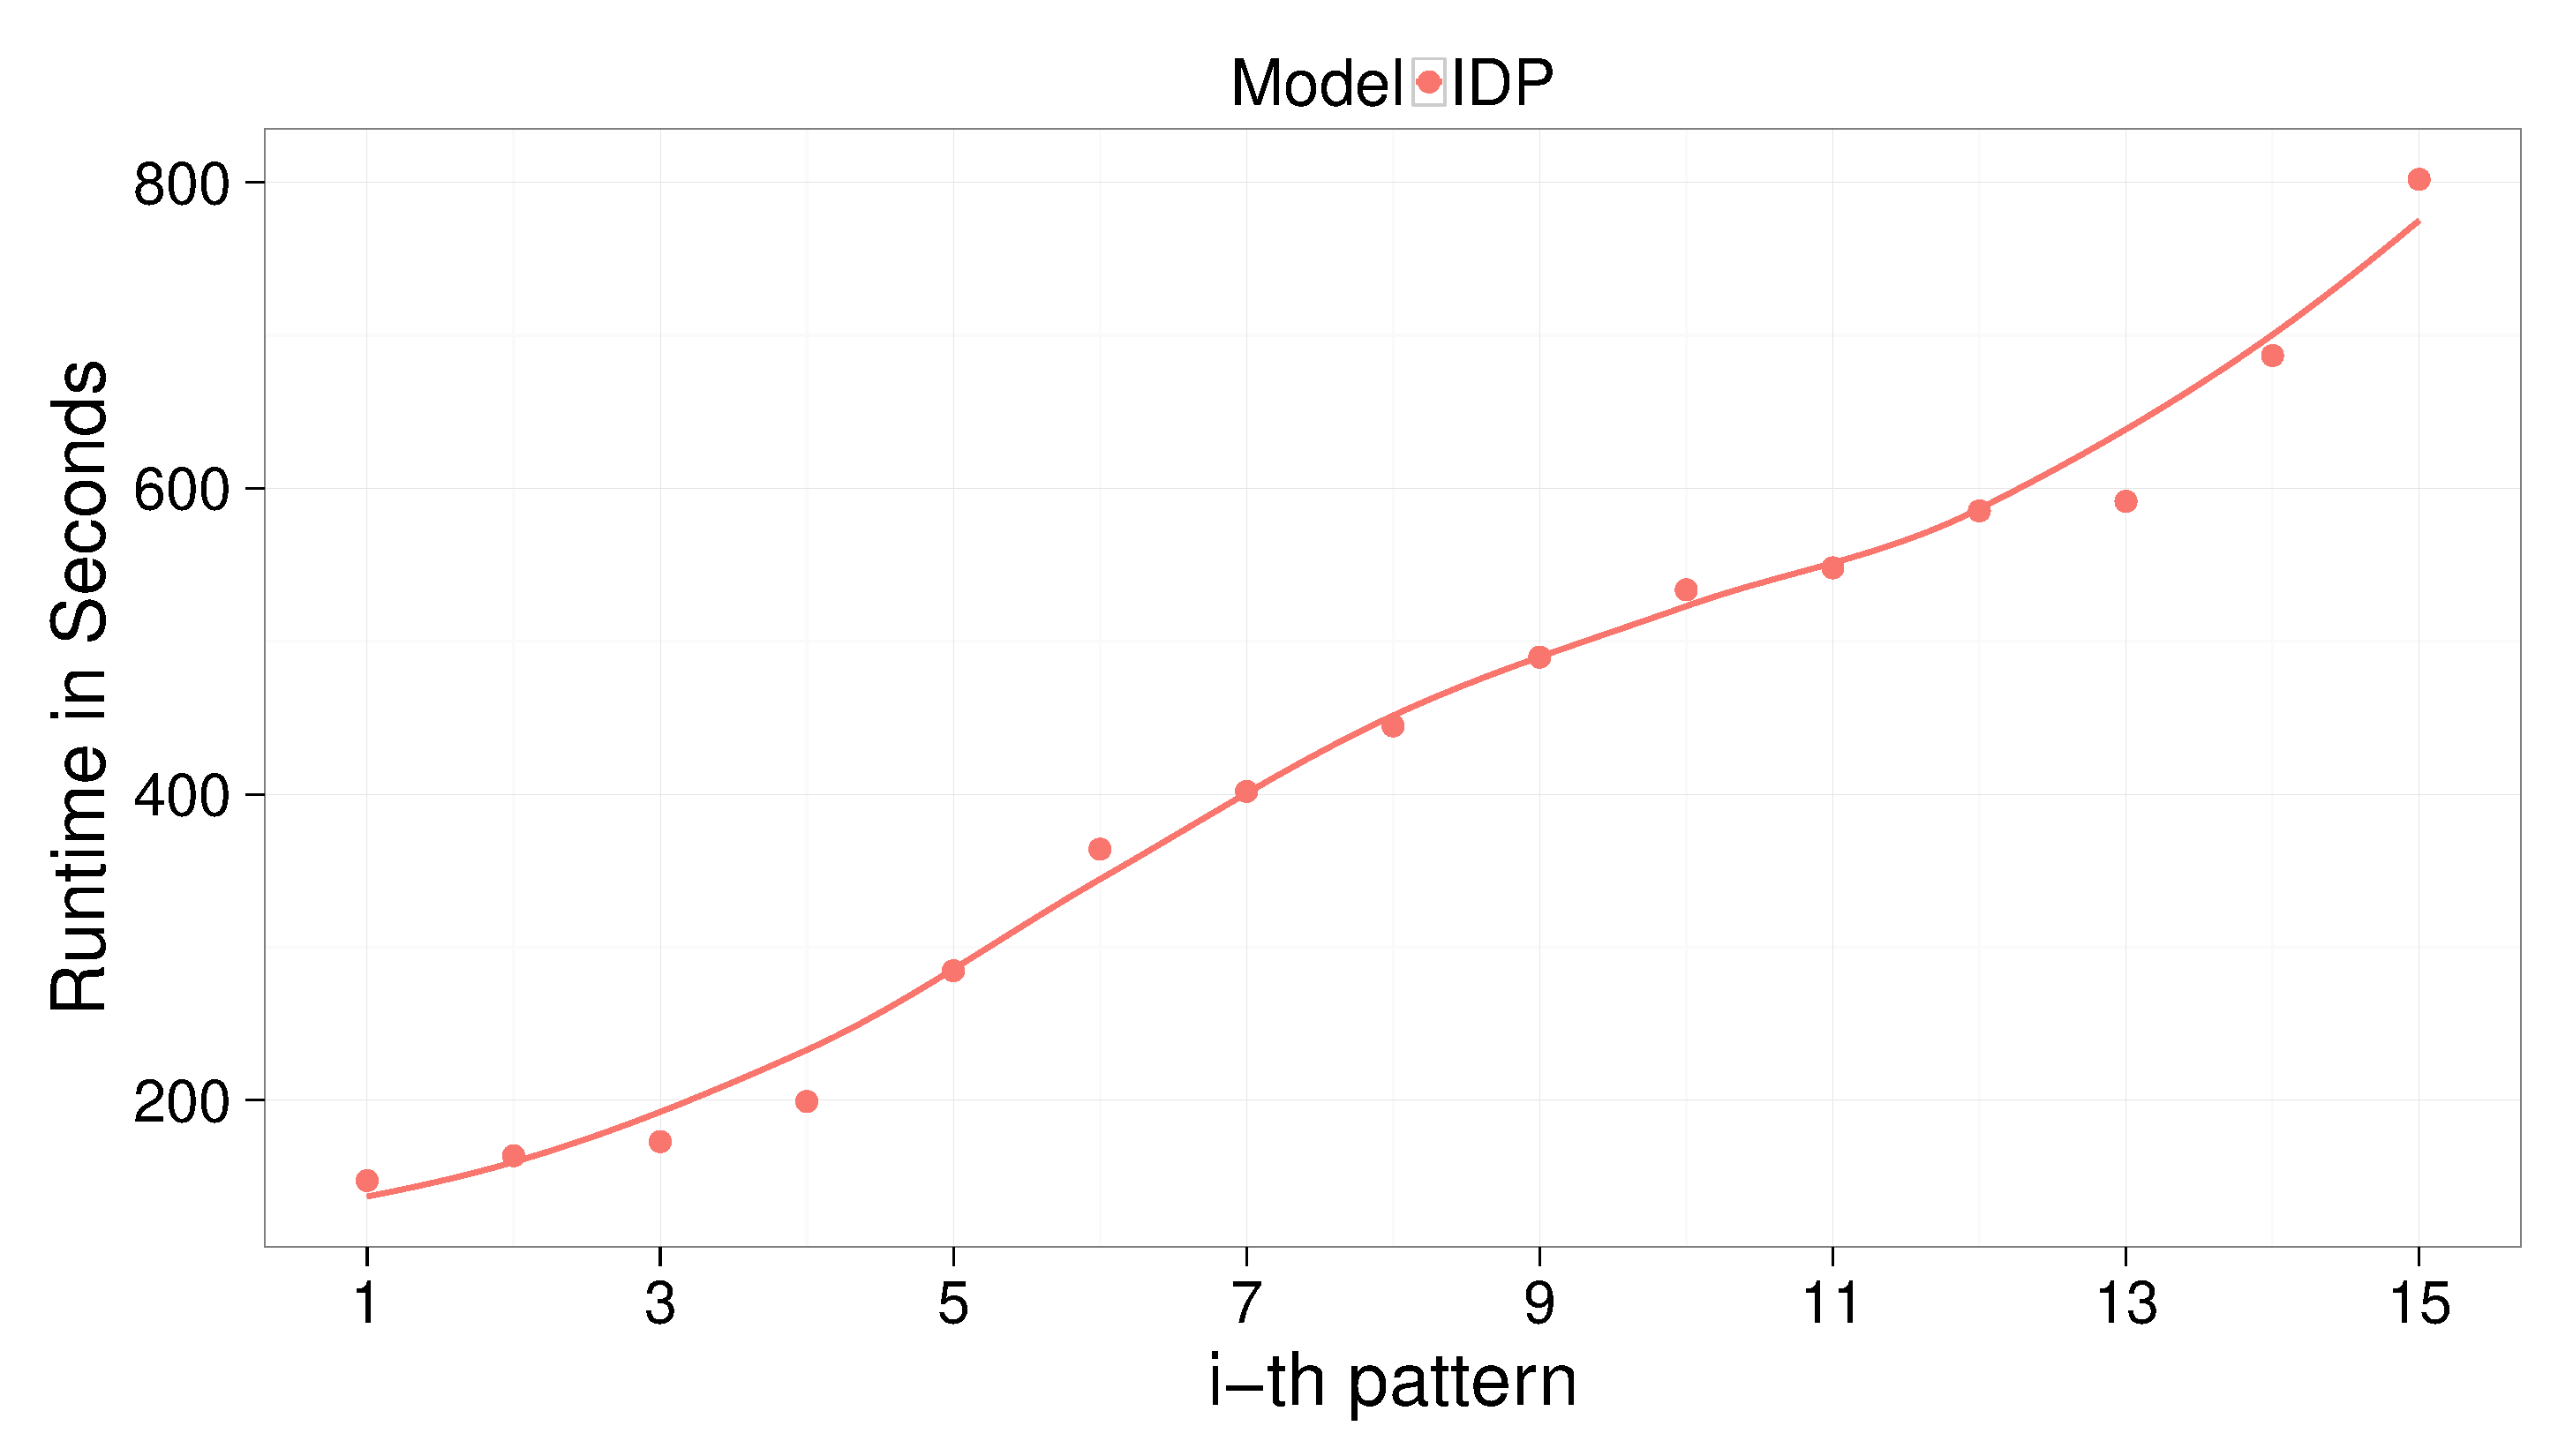
\includegraphics[scale=0.14]{extra/idp_prob_comparison.pdf}
% \caption{\footnotesize{Comparison between ProB (blue) and IDP (red) for the general graph mining problem on the Yoshida dataset} }
% \label{fig:ProBIDPComp}
% \end{figure}
% \sergey{to complete}

To analyze the effect of the disjoint union technique, we compared the performance of IDP and ASP on the Yoshida dataset using different encodings of the graph mining problem.
In \textbf{Fig.}~\ref{fig:decomposition_fol}, we see the performance of IDP (\textbf{Fig.}~\ref{fig:decomposition_idp}) and ASP (\textbf{Fig.}~\ref{fig:decomposition_asp}) on finding the $i$-th pattern.
Two different encodings are used: one that uses the disjoint union technique, and one that performs a new IDP/ASP call for every different example graph, and aggregates this data using procedural code (i.e. in a decomposed fashion).

It is clear from \textbf{Fig.}~\ref{fig:decomposition_fol} and the order(s) of magnitude difference between the decomposition and disjoint union technique that these systems can highly benefit from detecting the independence of these different subproblems and solving them separately.
We expect that expressing the problems in a higher order fashion will allow detection of this subproblem independence and allow for more performant and expressive systems.
\begin{figure}[thb]
\vspace{-2em}
\centering
\begin{subfigure}{.44\textwidth}
  \centering
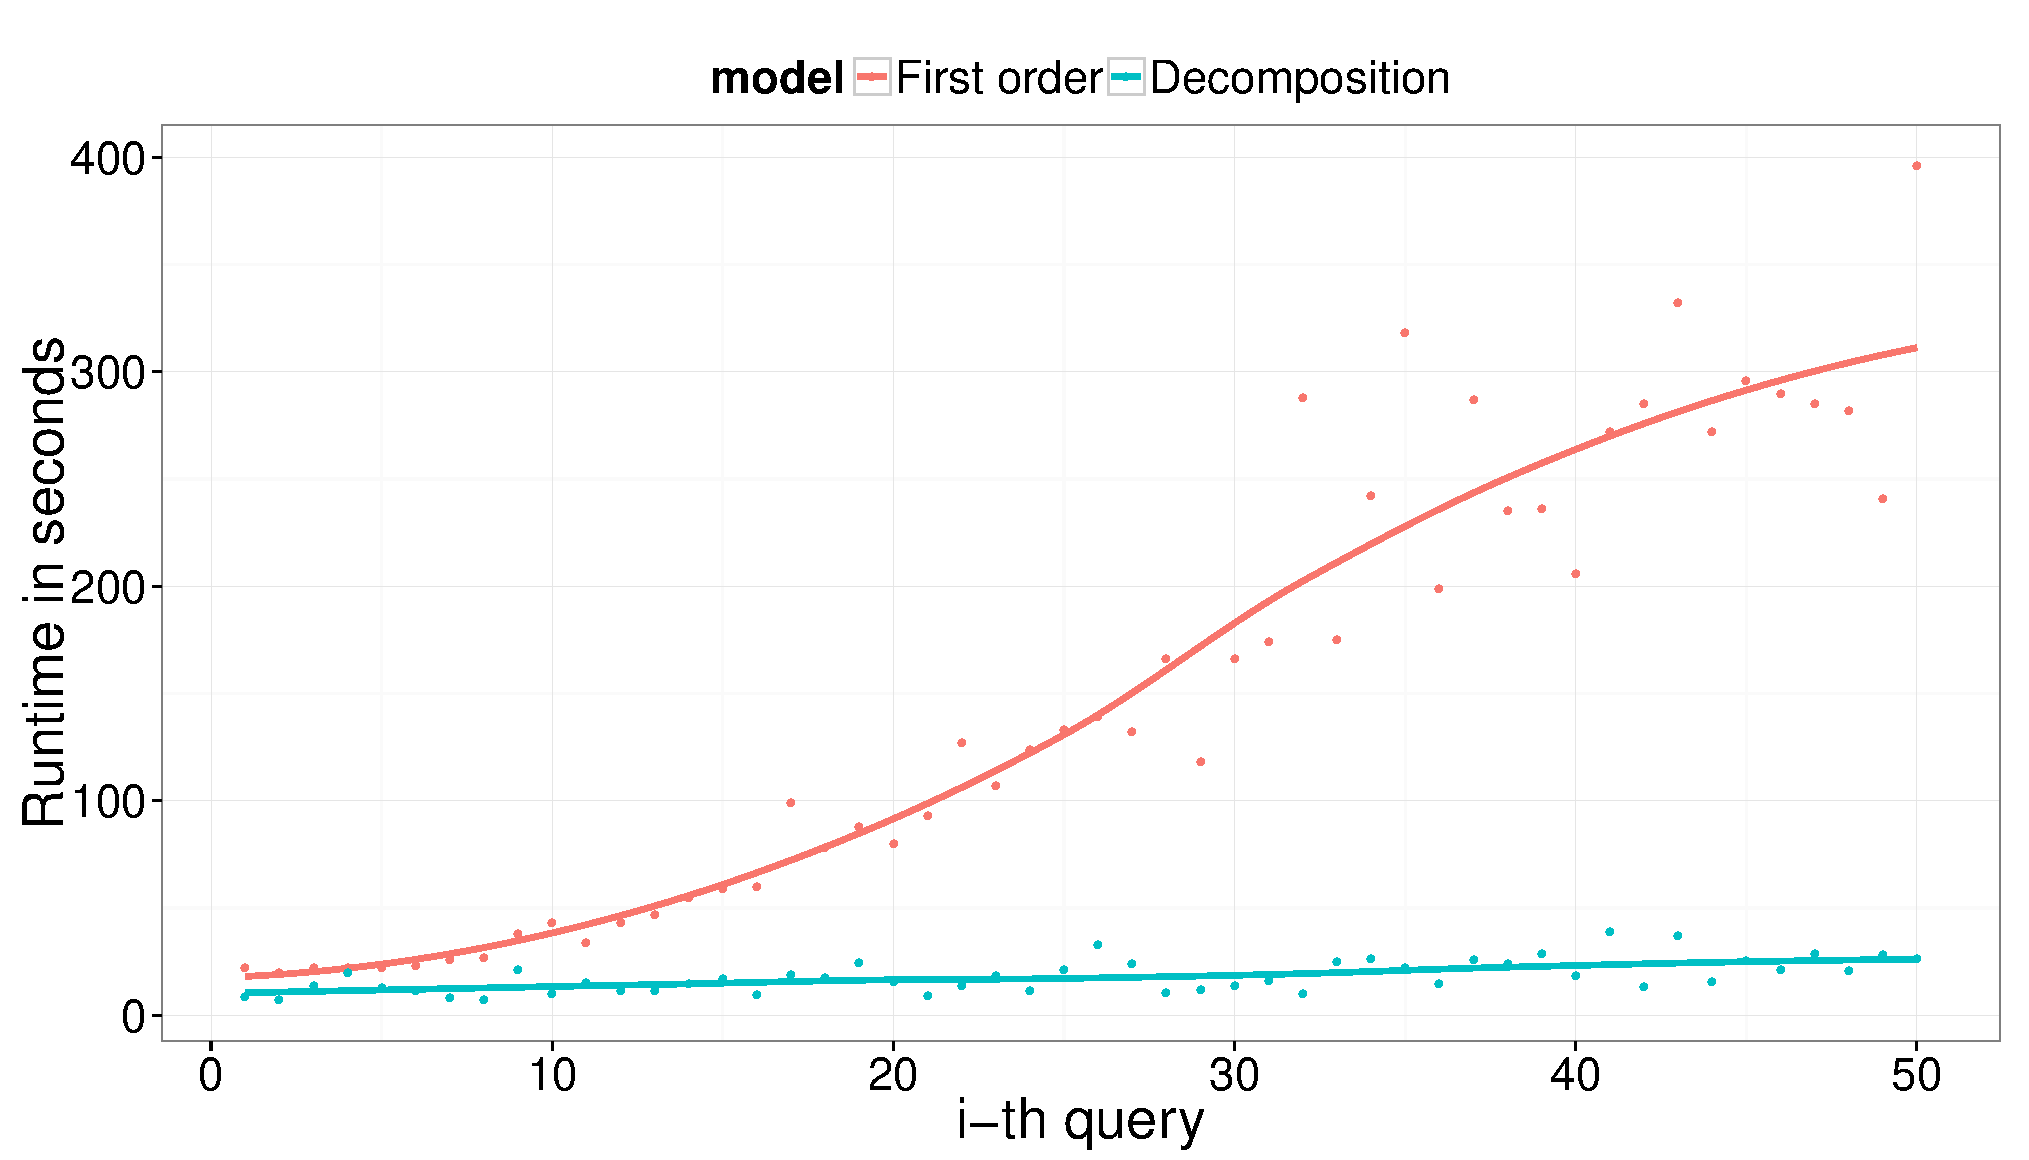
\includegraphics[scale=0.14]{extra/figure_comparison_yoshida.pdf}
\caption{\footnotesize{IDP: the disjoint model has a growing trend while the simulation stays flat. The gap is one order of magnitude. (\cite{ilp_graph_mining})}}
  \label{fig:decomposition_idp}
\end{subfigure}%
\hfill
\begin{subfigure}{0.46\textwidth}
  \centering
 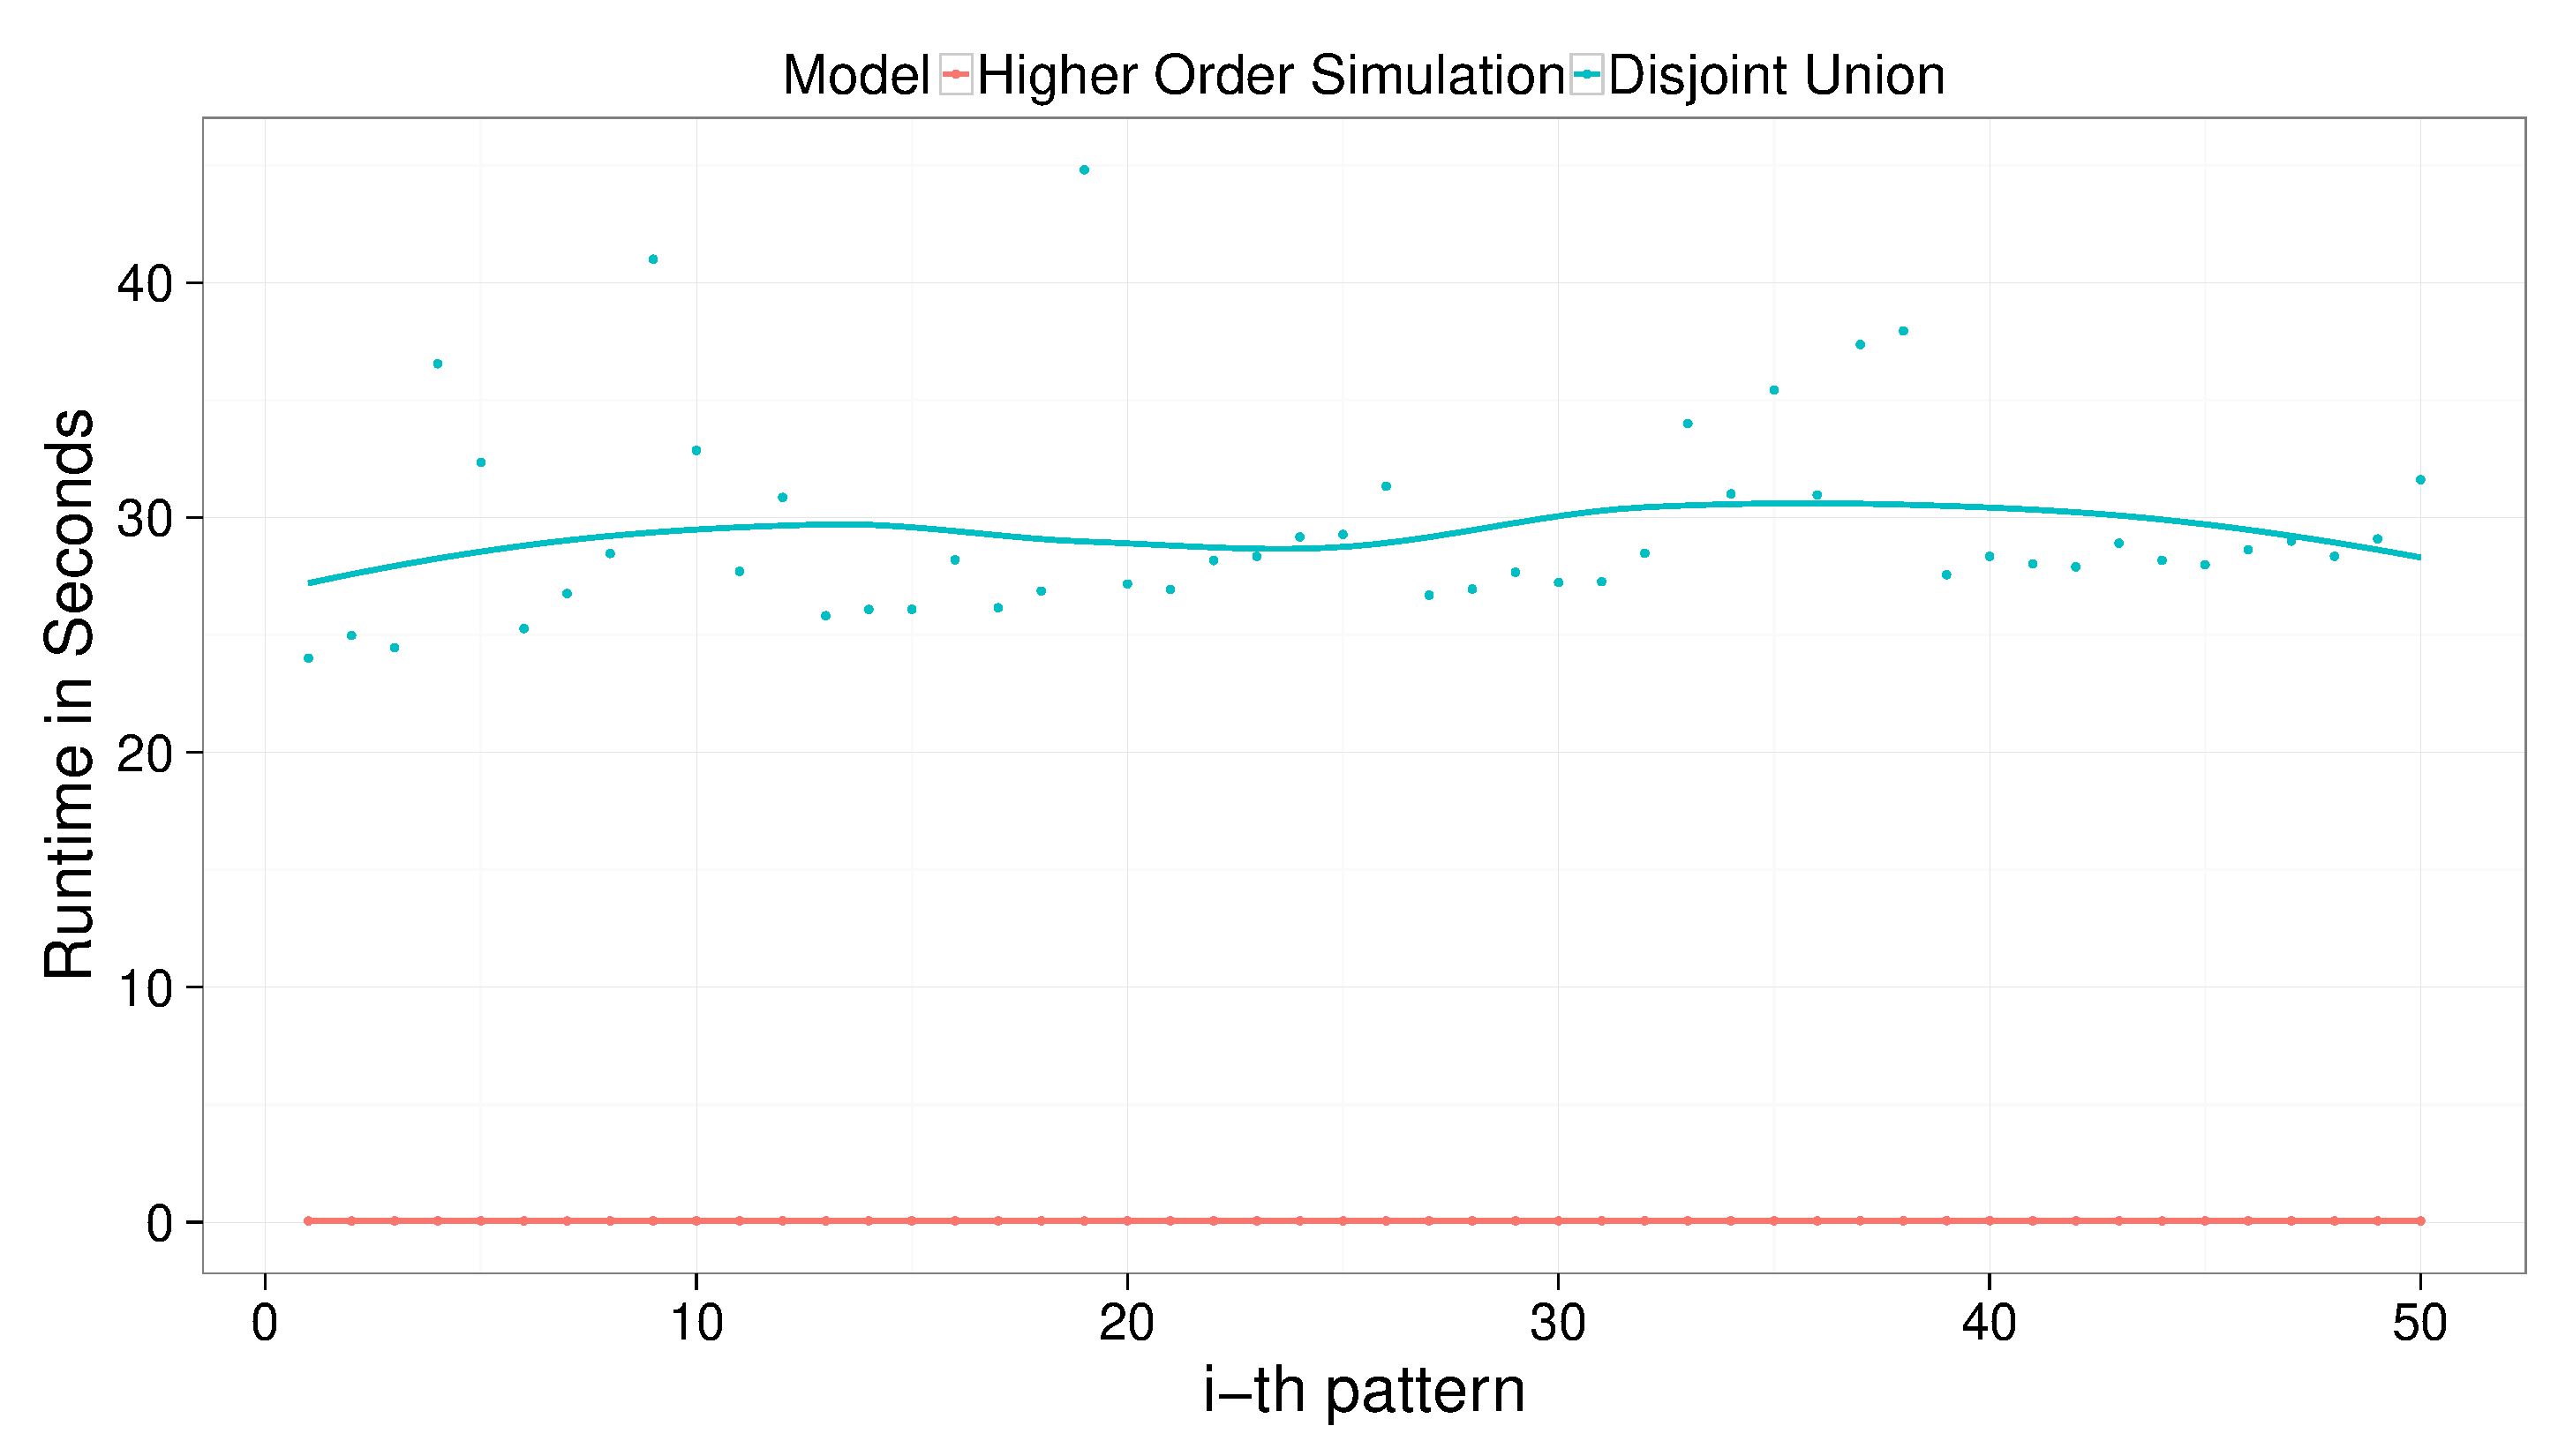
\includegraphics[scale=0.14]{extra/asp_fol_vs_decomposed_yoshida.pdf}
 \caption{\footnotesize{ASP: the disjoint model exhibits fluctuation around 30s with a slow runtime growth, while the simulation stays flat. The gap is two orders of magnitude.}}
  \label{fig:decomposition_asp}
\end{subfigure}
\caption{\footnotesize{Frequent graph enumeration problem (5\% threshold) on Yoshida dataset for IDP (a) and ASP (b), comparing disjoint union (in blue) and higher order simulations (in red). Further details can be found in \ref{sec:hol_description}.}}
\label{fig:decomposition_fol}
\end{figure}